\chapter{\IfLanguageName{dutch}{Resultaat}{Results}}
\label{ch:results}
\section{Metric outcome}
In this thesis we are measuring a couple of factors to see what the improvements are using micro frontends as opposed to the currently in place monorepo.

\subsection{Improvements for the developer}
Starting with the simplest to measure metric, the build times between the applications.
This metrics shows how much faster the micro frontend application builds and is ready to be tested by the developer. In our measures of building the CRM widget micro frontend application about 10 times, the average build speed is about 1 minute and 3 seconds. When the web application is built this takes about 4 minutes and 11 seconds on average. Seeing this there is an improvement of nearly 400\%. This means developers have to wait only a fourth of the time that they are used to and will be way faster in getting to test their written code.

\begin{table}
    \centering
    \begin{tabular}{|c|c|}
        \hline
        & Average build time \\ [1ex] 
        \hline\hline
        Monorepo & 4' 11'' \\  [1ex]
        \hline
        Micro Frontend & 1' 2'' \\[1ex]
        \hline
        Difference & 3' 8''  \\ [1ex] 
        \hline
        \multicolumn{2}{| c |}{Performance improvement of 400\%}\\
        \hline
    \end{tabular}
    
    \caption{Build times}
\end{table}

\subsection{Improvements for CI/CD}
As the pipeline for the micro frontend application was not finished yet, a simulation was made to get an idea of what the improvements would be in pipeline finishing speeds. The pipeline that is in place nowadays runs and tests the whole application as opposed to the future pipeline that would only run those checks for the specific micro frontend application. For this simulation a closer look was taken at all the pipeline checks and only those that were relevant to the micro frontend application were kept when the pipeline was run. The end-to-end tests were also excluded from both pipelines because they take the longest and will be removed in the future anyways. Of course this is not a 100\% accurate representation of what the true potential is in the future. But with our simulation we can already see some improvements.

The average time it takes for the entire pipeline with all its checks, tests, build and deploy times is 35 minutes and 29 seconds. The pipeline customized for the micro frontend application takes an average of 27 minutes and 51 seconds. As the data shows this is already an improvement of 7 minutes and 38 seconds. This accounts for an improvement of 27\%. Since the micro frontend initiative is still new within Showpad those times can still drastically improve. This simulation shows already good improvement but the true potential will be shown in the future when the actual pipeline is finished.

\begin{table}
    \centering
    \begin{tabular}{|c|c|c|c|}
        \hline
         & Tests \& Checks & Build \& Deploy & Total time \\ [1ex] 
        \hline\hline
        Monorepo & 21' 26'' & 14' 03`` & 35' 29`` \\ [1ex]
        \hline
        Micro Frontend & 17' 34`` & 10' 17`` & 27' 51`` \\[1ex]
        \hline
        Difference & 3' 52`` & 3' 46`` & 7' 38`` \\ [1ex] 
        \hline
         \multicolumn{4}{| c |}{Performance improvement of 27\%}\\
         \hline
    \end{tabular}
   
    \caption{Time to complete the CI/CD pipeline}
\end{table}

\subsection{Improvements in cycle time}
The most important metric is towards the user of the product. So how much has the micro frontend architecture an effect on how fast the user can have his hands on new features and fixes. 

For this metric it is important to understand that the currently main time losing factor within the process of getting code to production is being dependent on other teams. Since the current process of getting code to production is:

\begin{enumerate}
\item Writing code
\item Merging it into master through the pipeline
\item Testing in a staging environment
\item Waiting for one of the two deployments a day into production
\item Deploying
\end{enumerate}

Step 4 is the biggest time waster since all teams have to wait to deploy their code together. Deployments are currently scheduled to happen twice a day for the entire Showpad web application. In a micro frontend environment this wait time is completely eliminated because teams are no longer dependent on each other. Every team has their own micro frontend application which can be deployed to production whenever the team is ready to do so. So a team could hypothetically deploy 16 times a day if they really wanted to. This improves the cycle time so immensely it would not even be comparable.

\begin{figure}[!h]
    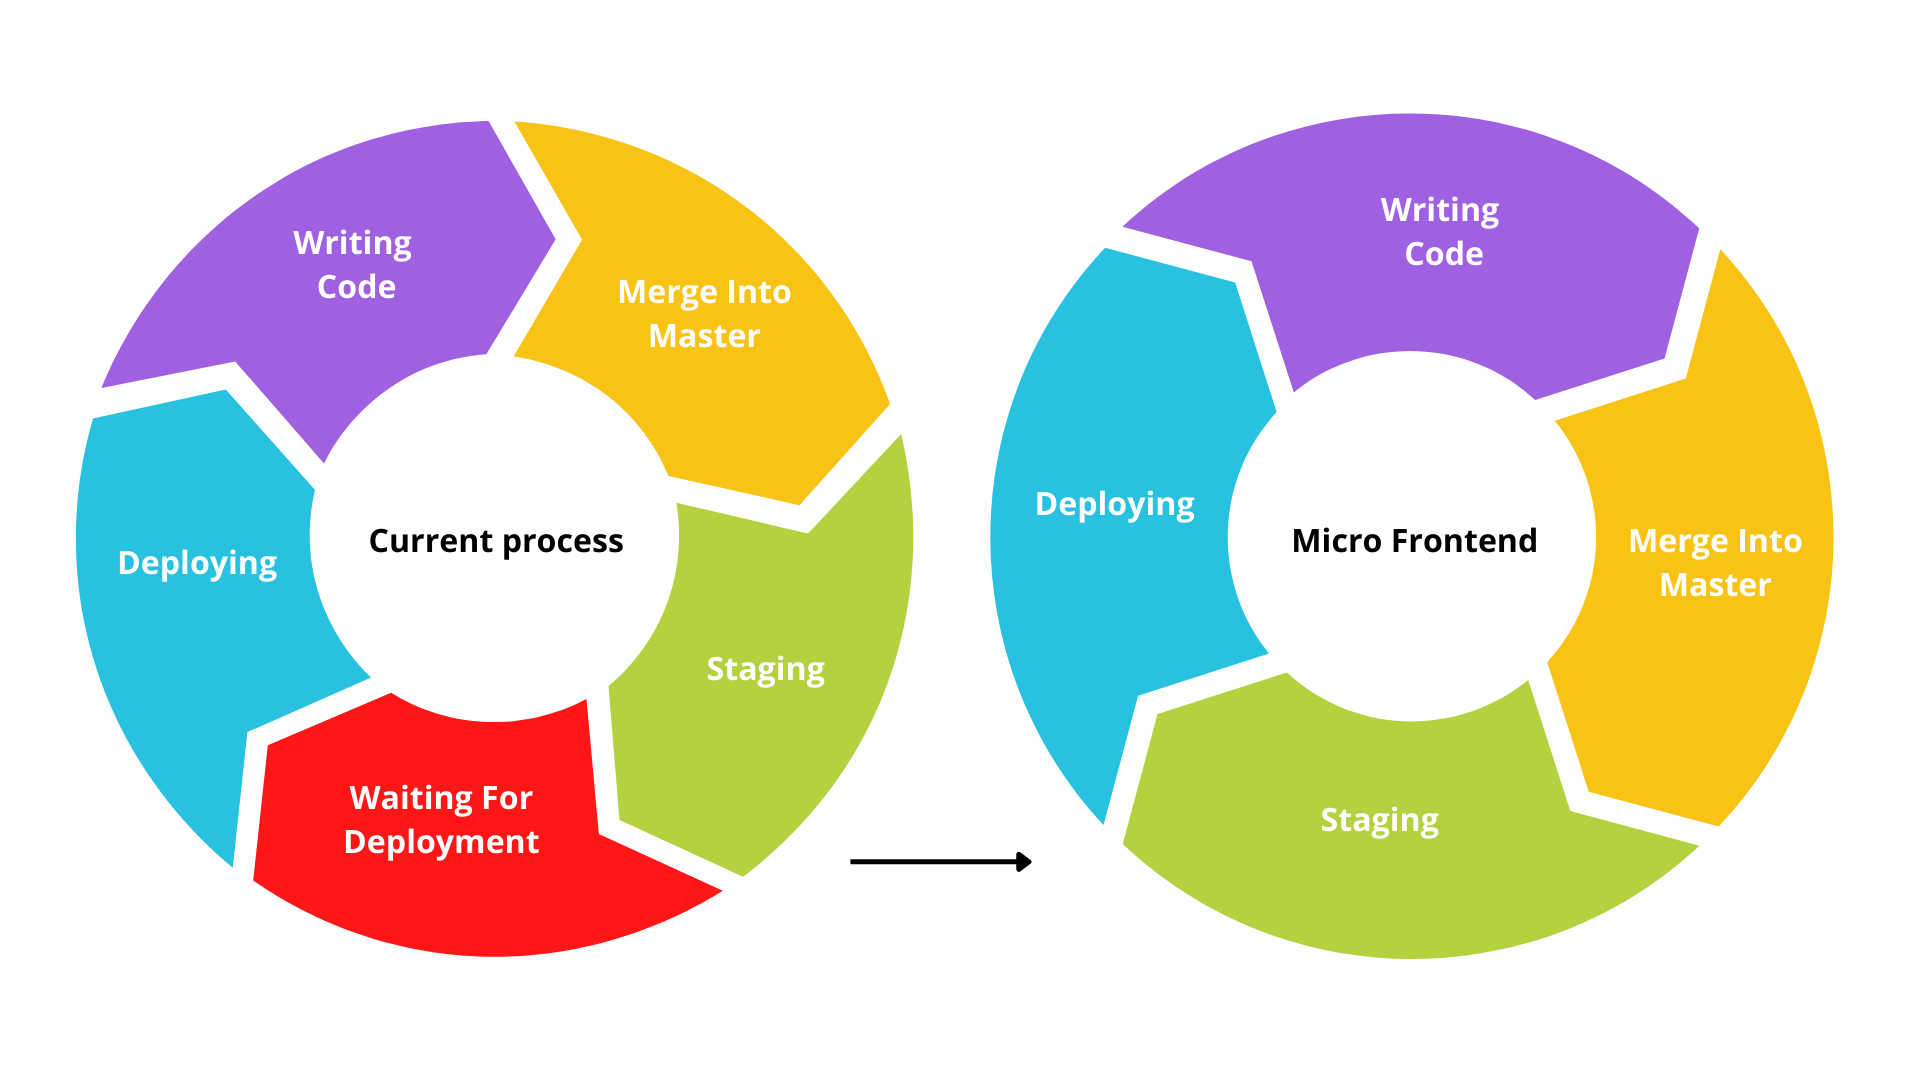
\includegraphics[width=12cm]{cyclus}
    \centering
\end{figure}
